%%%%%%%%%%%%%%%%%%%%%%%%%%%
%% Document is an article for a4 paper
\documentclass[a4paper]{article}
%% Encoding is utf8
\usepackage[utf8]{inputenc}
%% Fonts
\usepackage[T1]{fontenc}
%% Include graphic.
\usepackage{graphicx}
%% Use PGF to draw.
\usepackage{tikz}
%% Use tabularx
\usepackage{tabularx}
\usepackage{array}
%% Babel package
\usepackage[english]{babel}
%% Bit fields: to create message descriptions
\usepackage[bitheight=6ex]{bytefield}
%% Use hyper reference.
\usepackage[bookmarksopen=true]{hyperref}
\hypersetup{%
pdftitle={Share Resource},
pdfauthor={Anthony Jaguenaud},
pdfsubject={Share resource},
pdfkeywords={}}
%% Setup links.
\definecolor{darkred}{rgb}{0.5,0,0}
\definecolor{darkgreen}{rgb}{0,0.3,0}
\definecolor{darkblue}{rgb}{0,0,0.5}
\definecolor{darkbrown}{rgb}{0.28,0.07,0.07}

\hypersetup{%
  colorlinks=true,
  citecolor=darkblue,
  urlcolor=darkgreen,
  linkcolor=darkred,
  menucolor=darkbrown}

\newcommand{\field}[4]{
  \begin{tabular}{|p{3.5cm}|c|m{1cm}|m{2cm}|}
   \cline{1-1} \cline{3-4}
   #1 & \hspace{4cm} & #2 & #3 \\
   \hline
   \multicolumn{4}{|p{\textwidth}|}{#4} \\
   \hline
  \end{tabular}
}

\newcommand{\bitfield}[1]
{
    \begin{rightwordgroup}{Type\\\texttt{#1}}
      \wordbox{1}{\centering \texttt{#1}}
    \end{rightwordgroup} \\
}
\newcommand{\colorbitbox}[3]{%
\rlap{\bitbox{#2}{\color{#1}\rule{\width}{\height}}}%
\bitbox{#2}{#3}}

\newcommand{\SHABitboxes}{\bitbox{8}{[0]}
      \bitbox{8}{[1]}
      \bitbox{16}{\dots} \\
      \skippedwords \\
      \bitbox{16}{\dots}
      \bitbox{8}{[38]}
      \bitbox{8}{[39]}}

%\field{Header index}{Version}{Optional}{Header index is used to help to get information faster than reading fields one by one}
% \newcommand{\field}[4]{
%   \begin{tikzpicture}
%     \node (name) {#1};
%     \node (opt) {#2};
%     \node (version) [left = of opt] {#3};
%     \node (description) {#4};
%   \end{tikzpicture}
%
% }
% \newcommand{\field}[4]{
%   \begin{tabular}{|c|c|c|c|}
%   \cline{1-1}
%   #2 \\
%   \hline
%   \multirow{2}{*}{\rotatebox{90}{#1 }} & \multicolumn{3}{m{10cm}|}{#4} \\
%   \cline{2-4}
%   & \multicolumn{2}{c|}{#3} \\
%   \cline{1-3}
%   \end{tabular}
% }

\begin{document}
 \tableofcontents
 \section{Data format}
 \subsection{Directory and file organisation}
  \usetikzlibrary{trees}
\tikzstyle{every node}=[draw=black,thick,anchor=west]
\tikzstyle{selected}=[draw=red,fill=red!30]
\tikzstyle{optional}=[dashed,fill=gray!50]
\begin{tikzpicture}[%
  grow via three points={one child at (0.5,-0.7) and
  two children at (0.5,-0.7) and (0.5,-1.4)},
  edge from parent path={(\tikzparentnode.south) |- (\tikzchildnode.west)}]
  \node {root}
    child { node {04}
      child { node {\textbf{04}d528475b8f8dfb46107fc2fc98af2a2bc61ae1}}
    }
    child [missing] {}
    child { node {24}
      child { node {\textbf{24}80894a41445612d1cd7e1cb373598bd0500cc4}}
    }
    child [missing] {}
    child { node {40}
      child { node {\textbf{40}437af82bdcfa5122d6e592141b859888d07451}}
      child { node {\textbf{40}b69804e80e0192f041e964b0656d3ad8d3313e}}
    }
    child [missing] {}
    child [missing] {}
    child { node {6e}
      child { node {\textbf{6e}3be75e3b315c5a1ad32b23f76613b13e76aef9}}
    }
    child [missing] {}
    child { node {e6}
      child { node {\textbf{e6}3e3d1d2d7936278cab8d220dab6561db0c36e1}}
    }
    child [missing] {}
    child { node {fa}
      child { node {\textbf{fa}81dae4271daa04a584a77cf6ce721f42dd324d}}
    }
    child [missing] {}
    child { node {ff}
      child { node {\textbf{ff}085fda1d08567803896de7bb70b0dfc4b15383}}
    };

\end{tikzpicture}
\tikzstyle{every node}=[]

  Files are store in a directory.
Files represents Meta data storage units, or Data storage units.
Files are parts of a global resource.
We degign by “\emph{root}” directory the base directory use for storage.
The storage unit class, performs an SHA1 sum and set the name of the resource with this sum.
The first two characters of name are used to hash the files in \emph{root} directory.
The file name is not truncated in the subdirectory.
So, the first two characters of files in a subdirectory are the same for all files.

\begin{tabular}{|c|c|c|}
 \hline
 {Variable} & {Description} & {Default value} \\
 \hline
 \emph{Root} & Root directory of storage units. & \~/.local/share/CapProject/shareLib/ \\
 \hline
\end{tabular}

 \subsection{Meta Units format}
  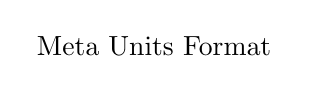
\begin{tikzpicture}
 \path (1,1) node{Meta Units Format};
\end{tikzpicture}


  Meta data unit have a particular format.
The first bytes of the file contain \emph{RS-META}\footnote{This is a 0 string terminated. So there are 8 characters reserved.}.
Then start real contain.
See Figure~\ref{fig:META-FILE-FORMAT} for more detail.
The next 8 bytes are the same than 8 first.
\begin{itemize}
 \item If the bytes in range [8..15] are not the same than in range [0..7] that means file is encrypted.
The key is not store by Share Resource library.
User software must delegate a key and the library will search the meta units that unlock.
The key is a symetric key.
 \item If the bytes in range [8..15] are the same than in range [0..7] that means unit is not encrypted.
\end{itemize}
\begin{figure}[htbp]
  \centering
\begin{bytefield}[bitwidth=2em]{16}
    \bitheader{0,7-8,15} \\

    \begin{rightwordgroup}{file header}
      % We have to do the \parbox explicitly in the next line because
      % \hyperlink typesets its argument in horizontal mode.\parbox{\width}{}
      \bitbox{1}{R} &
      \bitbox{1}{S} &
      \bitbox{1}{-} &
      \bitbox{1}{M} &
      \bitbox{1}{E} &
      \bitbox{1}{T} &
      \bitbox{1}{A} &
      \bitbox{1}{\textbackslash 0} &
      \bitbox{1}{R} &
      \bitbox{1}{S} &
      \bitbox{1}{-} &
      \bitbox{1}{M} &
      \bitbox{1}{E} &
      \bitbox{1}{T} &
      \bitbox{1}{A} &
      \bitbox{1}{\textbackslash 0}
   \end{rightwordgroup} \\

  \begin{rightwordgroup}{Meta data}
    \wordbox{2}{First meta field object\\ Should be \hyperlink{fields:meta-version}{Meta version}} \\
    \wordbox[lrt]{1}{%
      \parbox{0.6\width}{\centering (Meta field objects)}} \\
    \skippedwords \\
    \wordbox{2}{Last meta field object}
  \end{rightwordgroup}
  \end{bytefield}
  \caption{META file format.}
  \label{fig:META-FILE-FORMAT}
  \end{figure}




Data in the \emph{META unit} are serialized\footnote{That means that data can be stored with no order.}.

Each field have the same scheme (Figure~\ref{fig:META-FIELD-FORMAT}):

\begin{figure}[htbp]
  \centering
  \begin{bytefield}{32}
    \bitheader{0,7-8,15-16,23-24,31} \\

    \begin{rightwordgroup}{header}
      % We have to do the \parbox explicitly in the next line because
      % \hyperlink typesets its argument in horizontal mode.\parbox{\width}{}
      \wordbox{1}{\hyperlink{META-FIELD-Size}{\centering Size}} \\
      \wordbox{1}{\hyperlink{META-FIELD-Type}{type}}
    \end{rightwordgroup} \\

    \begin{rightwordgroup}{Object}
      \wordbox[lrt]{1}{%
        \parbox{0.6\width}{\centering (Object contain.)}} \\
      \skippedwords \\
      \wordbox[lrb]{1}{}
    \end{rightwordgroup}
  \end{bytefield}
  \caption{META object field.}
  \label{fig:META-FIELD-FORMAT}
\end{figure}


\begin{itemize}
  \item \hypertarget{META-FIELD-Size}{Size} of the object in byte. This include header, for a nul size object the size is 8.
  \item \hypertarget{META-FIELD-Type}{Type} of the object. Can be \emph{ResourceId} for example.
        All types are listed at the \hyperlink{META-FIELD-All-Types}{here}.
\end{itemize}







 \subsection{Data Units format}
  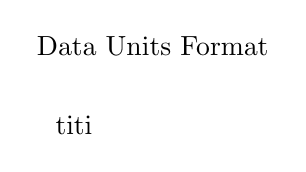
\begin{tikzpicture}
 \path (1,1) node{Data Units Format};
 \node (toto) at (0,0) {titi};
\end{tikzpicture}


  Data format.
\end{document}
